\documentclass{standalone}

% graphics
\usepackage{tikz}
\usepackage{pgfplots}
\usepackage{siunitx}

\begin{document}

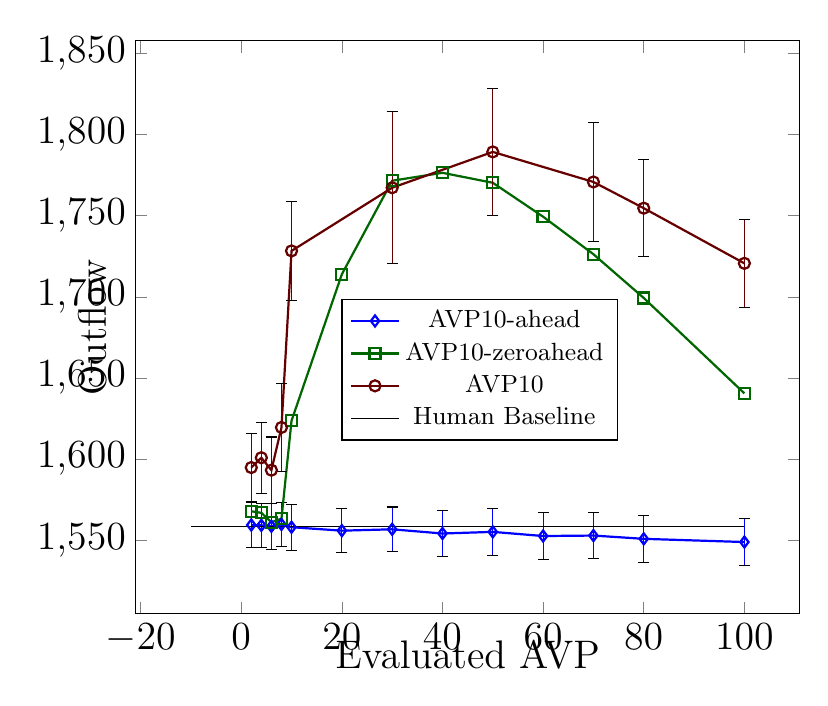
\begin{tikzpicture}[scale=1]
  \pgfplotsset{
      scale only axis,
      every x tick label/.append style={font=\Large},
      every y tick label/.append style={font=\Large},
	legend style={at={(0.31,0.55)},anchor=north west}
  }

\begin{axis}[
    legend style={font=\small},
	ylabel={\Large Outflow},
	x label style={at={(axis description cs:0.5,-0.03)},anchor=north},
	y label style={at={(axis description cs:-0.030,0.5)}, anchor=south},
	xlabel={\Large Evaluated AVP},
]


% trained on avp=10 
% dashdotdotted,
\addplot[mark=diamond, thick, mark options={solid, fill=blue!40, mark size=2 pt}, draw=blue, error bars/.cd, y dir=both, y explicit] table [x=a, y=b, y error=c] {
a	b   	c
2 1559.30 13.78
4 1559.09 13.61
6 1558.51 14.13
8 1559.63 13.58
10 1557.94 14.25
20 1555.81 13.60
30 1556.64 13.76
40 1554.05 14.34
50 1555.06 14.60
60 1552.50 14.75
70 1552.79 14.09
80 1550.77 14.59
100 1548.79 14.74
};
\label{AVP10-ahead}

% trained on avp=10 countahead=0
% error bars/.cd, y dir=both, y explicit,
\addplot[mark=square, thick, mark options={solid, fill=green!60, mark size=2 pt}, draw=black!60!green] table [x=a, y=b] {
a	b   	c
2 1567.76 16.87
4 1566.79 17.71
6 1561.03 15.45
8 1563.19 17.07
10 1623.60 35.07
20 1713.92 46.65
30 1771.60 50.75
40 1776.49 48.35
50 1770.34 43.37
60 1749.42 40.76
70 1726.27 39.21
80 1699.31 44.36
100 1640.48 49.13
};
\label{AVP10-zeroahead}  

% trained on avp=10 no countahead
%densely dashed, 
\addplot[mark=o, thick, mark options={solid, fill=black!60!red, mark size=2pt}, draw=black!60!red, error bars/.cd, y dir=both, y explicit] table [x=a, y=b, y error=c] {
a	b   	c
2	1594.73	20.77
4 	1600.78 21.92	
6	1593.11 20.44
8	1619.46 27.24
10	1728.32 30.39
30 	1767.28 46.92
50	1789.38 39.06
70	1770.84 36.94
80	1754.68 29.82
100	1720.66 27.16
};
\label{AVP10}
%
%%densely dashed, 
%\addplot[mark=triangle, thick, loosely dotted, mark options={solid, fill=red!60, mark size=2pt}, draw=black!20!red, error bars/.cd, y dir=both, y explicit] table [x=a, y=b, y error=c] {
%a	b   	c
%2 1560.38 15.36
%4 1573.70 20.76
%6 1603.84 26.81
%8 1619.50 23.10
%10 1629.58 26.28
%30 1705.79 30.68
%50 1732.86 32.70
%70 1760.51 32.22
%80 1773.72 42.27
%100 1784.16 39.10
%};
%\label{AVP70}
%
%%densely dashed, 
%\addplot[mark=otimes, thick, mark options={solid, fill=red!60, mark size=2pt},
%draw=blue!10!green, error bars/.cd, y dir=both, y explicit] table [x=a, y=b, y error=c] {
%a	b   	c
%2 1600.38 18.04
%4 1620.00 20.58
%6 1639.12 28.21
%8 1660.36 28.22
%10 1683.40 32.37
%30 1743.80 29.74
%50 1763.89 34.40
%70 1779.23 35.21
%80 1786.46 36.61
%100 1792.98 28.63
%};
%\label{AVP90}


%%densely dashed, 
%\addplot[mark=otimes, thick, mark options={solid, fill=blue!60, mark size=2pt},
%draw=blue!10!red, error bars/.cd, y dir=both, y explicit] table [x=a, y=b, y error=c] {
%a	b   	c
%2 1555.34 14.31
%4 1549.33 15.07
%6 1546.63 13.90
%8 1543.46 17.07
%10 1541.63 15.80
%20 1526.54 13.30
%30 1514.05 16.60
%40 1497.74 17.34
%50 1480.25 25.14
%60 1505.88 29.33
%70 1517.33 30.85
%80 1516.57 28.51
%100 1501.63 36.18
%};
%\label{linearPPO}

\addplot[mark=none, black, samples=200] coordinates {(-10,1558.12)
(100,1558.12)};
\label{Baseline}


\addlegendimage{/pgfplots/refstyle=AVP10}
\addlegendentry{AVP10-ahead}

\addlegendimage{/pgfplots/refstyle=AVP30}
\addlegendentry{AVP10-zeroahead}

\addlegendimage{/pgfplots/refstyle=AVP50}
\addlegendentry{AVP10}

%\addlegendimage{/pgfplots/refstyle=AVP70}
%\addlegendentry{AVP70}
%
%\addlegendimage{/pgfplots/refstyle=AVP90}
%\addlegendentry{AVP90}

%\addlegendimage{/pgfplots/refstyle=linearPPO}
%\addlegendentry{linearPPOAVP10}

\addlegendimage{/pgfplots/refstyle=Baseline}
\addlegendentry{Human Baseline}




\end{axis}
\end{tikzpicture}

\end{document}

